%==============================================================================
% Sjabloon poster bachproef
%==============================================================================
% Gebaseerd op document class `a0poster' door Gerlinde Kettl en Matthias Weiser
% Aangepast voor gebruik aan HOGENT door Jens Buysse en Bert Van Vreckem

\documentclass[a0,portrait]{hogent-poster}

% Info over de opleiding
\course{Bachelorproef}
\studyprogramme{toegepaste informatica}
\academicyear{2023-2024}
\institution{Hogeschool Gent, Valentin Vaerwyckweg 1, 9000 Gent}

% Info over de bachelorproef
\title{Automatische documentatie generatie met behulp van LLM's voor ongedocumenteerde Python-projecten.}
% \subtitle{Ondertitel (eventueel)}
\author{Max Milan}
\email{Max.Milan@student.hogent.be}
\supervisor{Gertjan Bosteels}
\cosupervisor{Arne Pannemans (ML6)}

% Indien ingevuld, wordt deze informatie toegevoegd aan het einde van de
% abstract. Zet in commentaar als je dit niet wilt.
\specialisation{Ai \& Data Engineering}
\keywords{Large Language Model, Python, Documentatie}
% \projectrepo{https://github.com/user/repo}

\begin{document}

\maketitle

\begin{abstract}
Deze bachelorproef richt zich op het documenteren van ongedocumenteerde Python-projecten met behulp van Large Language Models (LLM's) om zo duidelijke en overzichtelijke documentatie te genereren.
De gegenereerde documentatie van een bestand, de docstrings en de bestandsamenvattingen worden als basis gebruikt voor de projectdocumentatie.
Deze projectdocumentatie bevat een samenvatting van alle bestanden en de relaties tussen deze bestanden.
De evaluatie van de automatisch gegenereerde documentatie toont aan dat de documentatie van de tool en de handgeschreven documentatie gelijkaardig zijn.
\end{abstract}

\begin{multicols}{2} % This is how many columns your poster will be broken into, a portrait poster is generally split into 2 columns

\section{Introductie}
Deze bachelorproef onderzoekt het documenteren van ongedocumenteerde Python-projecten met behulp van LLM's. 
De doelstelling is om een proof-of-concept te ontwikkelen dat de documentatie van een Pythonproject kan genereren op basis van de code.
Zodat de kennis makkelijk gedeeld kan worden en dat iedereen die met het project in aanraking komt, snel de nodige informatie kan vinden.

\section{Methodologie}
Het onderzoek bestaat uit 4 fases. Een literatuurstudie naar wat documentatie juist is en wat enkele bestaande tools zijn.
De volgende stap is het documenteren van bestanden met behulp van LLM's. Hierna volgt het genereren van Projectdocumentatie, een samenvatting van alle bestanden en relaties ertussen.
Als laatste wordt er een evaluatie gedaan van de automatische gegenereerde documentatie.

\section{Resultaten}
Het documenteren van een bestand gebeurt door uit de code functies en klassen te halen en mee te geven aan een prompt.
Op basis van de gegenereerde docstrings wordt er een samenvatting van het bestand gemaakt een voorbeeld hiervan is te zien in de figuur \ref{fig:bestanddocu}.

\begin{center}
  \captionsetup{type=figure}
  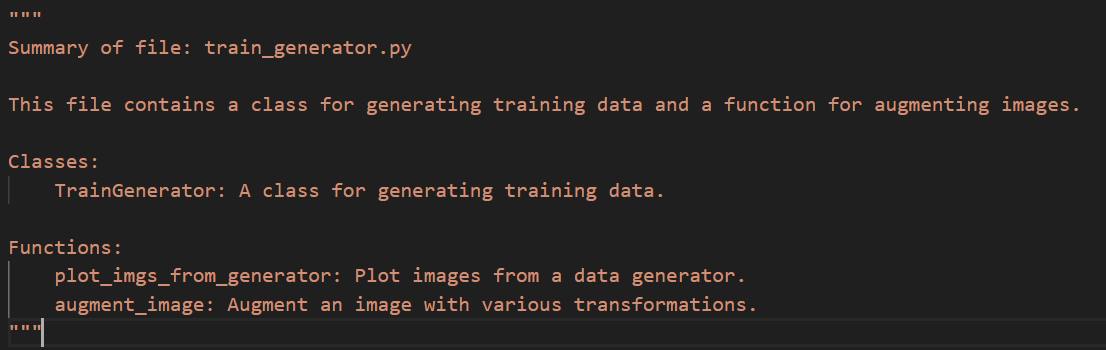
\includegraphics[width=1.0\linewidth]{auto_bestanddocu}
  \captionof{figure}{Automatisch gegenereerde documentatie van een bestand.}
  \label{fig:bestanddocu}
\end{center}

De documentatie van een project is een samenvatting van alle bestanden en de relaties tussen deze bestanden.
Alle bestanden worden gedocumenteerd en de bestandsamenvattingen worden omgezet tot één projectsamenvatting.
De relaties tussen de bestanden worden gevisualiseerd met behulp van een graaf en dit op basis van de imports in de bestanden en de bestandsnamen.
Een voorbeeld van een graaf met de relaties tussen de bestanden is te zien in figuur \ref{fig:graaf}.

\begin{center}
  \captionsetup{type=figure}
  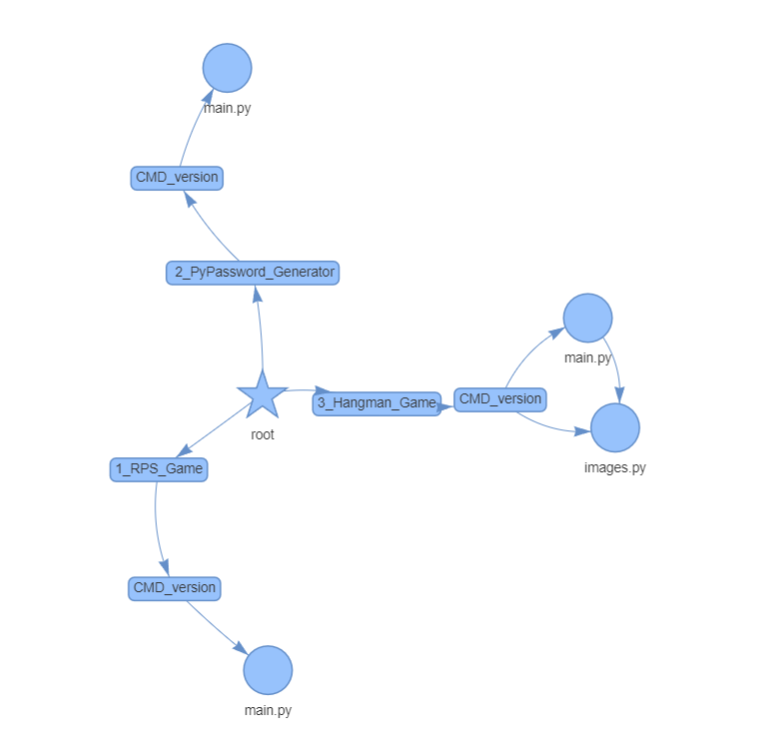
\includegraphics[width=0.8\linewidth]{graph}
  \captionof{figure}{Graaf met de relaties tussen de bestanden.}
  \label{fig:graaf}
\end{center}

\section{Evaluatie}

De evaluatie van de gegenereerde documentatie met manueel geschreven documentatie toont aan dat de automatisch gegenereerde documentatie een goede basis is.
De docstrings komen voor 90\% overeen met de manueel geschreven documentatie en de bestandsamenvattingen komen voor 62.5\% overeen met de manueel geschreven documentatie.

\section{Conclusies}
De evaluatie toont aan dat de documentatie van de tool en de handgeschreven documentatie gelijkaardig zijn. 
Alhoewel er enkele fouten in de documentatie van de individuele bestanden zitten, blijft
de gehele projectdocumentatie overzichtelijk en duidelijk.

\section{Toekomstig onderzoek}
Er kan gekeken worden naar een uitgebreidere evaluatie van de documentatie. 
Met een grote enquête en programmeurs manueel laten documenteren en deze te vergelijken met de automatisch gegenereerde documentatie.

\end{multicols}
\end{document}